\subsection{Agentes Racionais}
“Mas seria possível uma máquina pensar?“ Esse questionamento inicial de Turing, desencadeou a proposta do \textit{Imitation Game}, que basicamente consiste em colocar uma pessoa (1) para conversar com um computador, esse computador poderá ser uma inteligência artificial ou outra pessoa (2) conversando através da máquina. O objetivo é que a pessoa 1 consiga distinguir se quem esta conversando com ela é a máquina ou a pessoa 2. A proposta feita por Turing seria considerada como um agir humanamente. Ela baseia-se em criar uma máquina que reconhece a escrita, tome decisões a partir de um base de dados e por final seja capaz de se aprimorar diante de novos cenários. Porém, como seria desenvolvido algo de tal amplitude? A resposta é que “não seria”! Questionar se uma máquina é capaz de pensar seria o mesmo que questionar se um submarino é capaz de nadar, afirmou Dijsktra, apontando que o termo "pensar" e "nadar" tinham suas definições restritas, entretanto, era possível realizar ações similares tão bem quanto \cite[2-3]{dijkstra898, turing1950, russell2003artificial}.

Para realizar as ações descritas por Turing, é necessário entender os passos descritos por ele de forma racional e lógica afim de replicá-los para a máquina.

A abordagem de agentes racionais é uma das possibilidades a serem usadas. O termo racional significa algo baseado ou acordado com uma razão ou lógica, de outro lado, a lógica tem dois pilares: a conversão responsável por expressar a mesma proposição em diferentes formas e o silogismo responsável por localizar um termo em comum que conecte duas dessas proposições. Um agente é algo que age, ou seja, um agente racional seria quem analisa circustâncias utilizando de definições lógicas e racionais a fim de interagir com algo. Isso é afirmado pela definiçao de Russel\cite[7]{russell2003artificial}, onde um agente racional percebe modificações no ambiente, através de sensores, e interage de volta com o ele novamente através de atuadores. Pode-se notar esse fluxo na Figura \ref{fig:rational_agent_draw}.

Logo, é possivel afirmar, que para ser possível realizar ações racionais é necessário entender o ambiente aonde você esta e suas variáveis, alias, é necessário que esteja claro o que pode ou não ser computado, quais são as regras que se aplicam e principalmente como obter algo racional com base em informações abstratas ou com dados incompletos \cite{frege1956thought, wooldridge1994agent, simon1955behavioral, boole1854investigation, russell2003artificial}

\begin{figure}
    \centering
    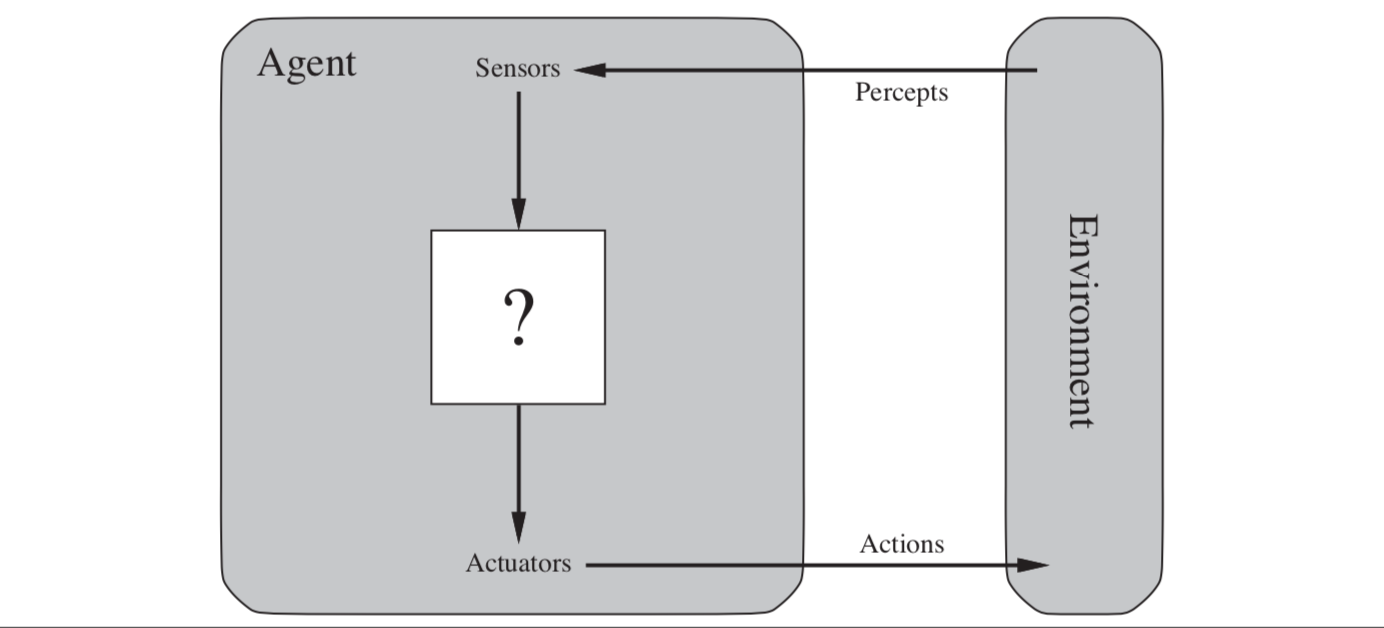
\includegraphics[width=.8\textwidth]{imagens/rational_agent_draw.png}
    \caption{Fluxo executado por um agente racional. Fonte: Russel, 2003, 35. Adaptada pelo Autor}
    \label{fig:rational_agent_draw}
\end{figure}

Definir se o agente está ou não gerando os dados esperados é um dos passos durante o desenvolvimento dos agentes. É necessário analisar o ambiente gerado a partir das percepções e conferir se os dados são os esperados ou não, essa etapa chama-se mensuração de \textit{performance}. Resumidamente, o agente receberá um entrada de dados e será responsável por gerar um saída. Ao longo do tempo o mesmo agente gerara múltiplas percepções e essas formarão uma sequencia de percepções \footnote{Não serão todos os modelos que seguirão a proposta sequencial, existem casos em que a linha temporal não afeta o desenvolvimento da decisões tornando-as episódicas}.

Existem vários tipos de agentes racionais, sendo definidos como \cite[34-45]{russell2003artificial}:

\begin{itemize}
 \item Totalmente, parcialmente ou não observador: essa definição é gerada pela quantidade de fatores do ambiente que seu agente recebe, um agente que tem todas as informações do ambiente é totalmente observador enquanto um que não recebe nada, precisando assim manter alguns estados, é não observador.
 \item Estocástico ou Determinístico: quando é impossível determinar o próximo estado através do anterior o agente é Estocástico, caso ao contrario ele é Determinístico.
 \item Episódicos ou Sequenciais: já foi dito que em diversas abordagens são gerados sequencias de percepção, quando essa sequencia é alterada a partir de alguma mudança de estado o agente é chamado de sequencial, caso ao contrario o agente é episódico.
 \item Estáticos ou Dinâmicos essa definição é referente ao ambiente, quando o ambiente não infere alterações o agente é nomeado estático, caso ao contrario Dinâmico.
 \item Continuo ou Distinto: Quando existem finitas possibilidades de estado pode se afirmar que o agente é Distinto, quando as possibilidades são infinitas é dado o nome de Continuo.
 \item Conhecido ou Desconhecido: Quando o agente necessita aprender algo e não consegue realizar a ação por si só ele é um agente desconhecido, caso contrário ele é conhecido.
\end{itemize}

Porém, é necessário diferenciar um agente racional de um algoritmo de tomada de decisão. O fato é que um agente pode tomar uma decisão, porém ele não gera só uma solução, mas sim, a equação necessária para conseguir essa solução. Além disso, baseado em um sistema inteligente com múltiplos agentes racionais, fica-se o questionamento sobre o quão inteligente um agente isolado pode ser, e também, quantos agente são necessários para que a máquina consiga obter o conhecimento desejado. Essas questões levam a IA para o próximo passo: ensinar um sistema a coletar esses resultados.
